%%
%% This is file `sample-sigconf.tex',
%% generated with the docstrip utility.
%%
%% The original source files were:
%%
%% samples.dtx  (with options: `sigconf')
%%
%% IMPORTANT NOTICE:
%%
%%% For the copyright see the source file.
%%
%% Any modified versions of this file must be renamed
%% with new filenames distinct from sample-sigconf.tex.
%%
%% For distribution of the original source see the terms
%% for copying and modification in the file samples.dtx.
%%
%% This generated file may be distributed as long as the
%% original source files, as listed above, are part of the
%% same distribution. (The sources need not necessarily be
%% in the same archive or directory.)
%%
%% The first command in your LaTeX source must be the \documentclass command.

% Modify this to remove all ACM and conference information (for arXiv for example)
\def\removeHeaders{no}

\def\tempYes{yes}
\def\tempNo{no}
\documentclass[10pt,sigconf,letterpaper,dvipsnames\ifx\removeHeaders\tempYes ,nonacm\fi]{acmart}
\acmYear{2019}
\copyrightyear{2019}
\acmConference{Workshop on Buffer Sizing}{December 2-3, 2019}{Stanford, California, USA}

\usepackage[utf8]{inputenc}

%\usepackage{multirow}
%\usepackage{blindtext}
%\usepackage{soul}
\usepackage{enumitem}
\usepackage{algorithmicx}
\usepackage{algpseudocode}
\usepackage{algorithm}
\usepackage{graphicx}
\usepackage{subfig}

% Acronyms
\usepackage[nomain, toc, acronym]{glossaries}
\glsdisablehyper

\ifx\removeHeaders\tempYes
\settopmatter{printacmref=false} % Removes citation information below abstract
\renewcommand\footnotetextcopyrightpermission[1]{} % removes footnote with conference information in first column
\fi

\newcommand\note[2]{{\color{#1}#2}}
\newcommand\todo[1]{{\note{red}{TODO: #1}}}

\makeatletter
\newcommand{\StateIndent}[1][3]{%
  \setlength\@tempdima{\algorithmicindent}%
  \Statex\hskip\dimexpr#1\@tempdima\relax}
\algdef{S}[WHILE]{WhileNoDo}[1]{\algorithmicwhile\ #1}%
\makeatother

\algnewcommand\True{\textbf{true}}
\algnewcommand\False{\textbf{false}}
\algnewcommand\Break{\textbf{break}}

\newcommand{\algorithmautorefname}{Algorithm}

%%
%% Submission ID.
%% Use this when submitting an article to a sponsored event. You'll
%% receive a unique submission ID from the organizers
%% of the event, and this ID should be used as the parameter to this command.
%%\acmSubmissionID{123-A56-BU3}

%%
%% The majority of ACM publications use numbered citations and
%% references.  The command \citestyle{authoryear} switches to the
%% "author year" style.
%%
%% If you are preparing content for an event
%% sponsored by ACM SIGGRAPH, you must use the "author year" style of
%% citations and references.
%% Uncommenting
%% the next command will enable that style.
%%\citestyle{acmauthoryear}

%%
%% end of the preamble, start of the body of the document source.
\begin{document}

%%
%% The "title" command has an optional parameter,
%% allowing the author to define a "short title" to be used in page headers.
\title{Congestion Control Aware Queuing}

%% GLOSSARY

\newacronym{aqm}{AQM}{Active Queue Management}
\newacronym{cc}{CC}{Congestion Control}
\newacronym{cca}{CCA}{Congestion Control Algorithm}
\newacronym{qdisc}{qdisc}{queuing discipline}
\newacronym{fq}{FQ}{Fair Queuing}
\newacronym{rtt}{RTT}{Round-Trip Time}
\newacronym{gi}{GI}{Guard Interval}
\newacronym{li}{LI}{Longest Interval}
\newacronym{bdp}{BDP}{Bandwidth Delay Product}

\begin{abstract}
Recent model-based congestion control algorithms such as BBR use repeated measurements at the end-point to build a model of the network connection and use it to achieve optimal throughput with low queuing delay. Conversely, applying this model-based approach to Active Queue Management (AQM) has so far been underinvestigated. We propose an AQM scheduler based on fair queuing, which adapts the buffer size depending on the needs of each flow without requiring active participation from the endpoint. We implement this scheduler for the Linux kernel and show that it interacts well with the most common congestion control algorithms and can significantly increase throughput compared to CoDeL while avoiding overbuffering.
\end{abstract}

%%
%% The "author" command and its associated commands are used to define
%% the authors and their affiliations.
%% Of note is the shared affiliation of the first two authors, and the
%% "authornote" and "authornotemark" commands
%% used to denote shared contribution to the research.
\author{Maximilian Bachl, Joachim Fabini, Tanja Zseby}
\affiliation{\institution{Technische Universität Wien}}
\email{firstname.lastname@tuwien.ac.at}


%%
%% By default, the full list of authors will be used in the page
%% headers. Often, this list is too long, and will overlap
%% other information printed in the page headers. This command allows
%% the author to define a more concise list
%% of authors' names for this purpose.
%\renewcommand{\shortauthors}{Hartl and Bachl}

%%
%% The abstract is a short summary of the work to be presented in the
%% article.
%\begin{abstract}
%  A clear and well-documented \LaTeX\ document is presented as an
%  article formatted for publication by ACM in a conference proceedings
%  or journal publication. Based on the ``acmart'' document class, this
%  article presents and explains many of the common variations, as well
%  as many of the formatting elements an author may use in the
%  preparation of the documentation of their work.
%\end{abstract}

\newcommand{\codel}{CoDeL}

\settopmatter{printfolios=true}
\maketitle

\section{Introduction}

In the last decades various \gls{aqm} mechanisms have been proposed to minimize excessive standing queues in the Internet. One of the most influential recent efforts is \codel{} \cite{nichols_controlling_2012} whose goal is that the queuing delay at the bottleneck link is at least once under 5\;ms in a moving window of 100\;ms. 

While it is important to keep the queuing delay constrained, it is also necessary to ensure that overly ``aggressive'' flows cannot benefit by ``stealing'' less aggressive flows' bandwidth. Thus researchers and engineers have developed \textit{\gls{fq}} mechanisms \cite{shreedhar_efficient_1996,dumazet_pkt_sched:_2013} to isolate different flows' queues so that for example a delay-sensitive live video call cannot be impaired by a concurrent bulk transfer which takes all the available bandwidth. 

Recent approaches have tried to combine \gls{aqm} with \gls{fq}. \cite{taht_flow_2018} demonstrate \textit{fq\_codel}, a \gls{qdisc} that uses \gls{fq} and lets \codel{} manage each queue. \cite{hoiland-jorgensen_piece_2018} expand upon this and create the \textit{cake} \gls{qdisc} that also adds features such as not only per-flow queuing but also per-host queuing for even increased fairness. Furthermore they also include bandwidth shaping into their solution and aim to create one \gls{qdisc} that is easy to configure and can be easily deployed on home routers and offers all features in one solution. 

While we do not want to make statements about the general performance of \codel{}, we show that fq\_codel and cake do not optimally use available bandwidth in common network configurations for common \glspl{cca}. This becomes especially prevalent for links with a high bandwidth or a large \gls{rtt} but is already noticeable for common scenarios, such as a link with 100\;Mbit/s and an \gls{rtt} of 50\;ms. 

We show that the impaired performance is a result of keeping the queuing delay under 5\;ms, which hinders \glspl{cca} such as Reno or Cubic from reaching maximum throughput. The problem is that these \glspl{qdisc} aim to keep the delay under the threshold no matter the effect on throughput and do not take the \gls{cc} of the flow into account. 

As a remedy, we conceive an \gls{aqm} mechanism that explicitly measures the behavior of the \gls{cc} of a flow and dynamically changes the buffer so that 
\begin{enumerate}[topsep=0pt,wide,labelwidth=!,labelindent=0pt]
\item link utilization is optimized and
\item queuing delay is kept at the minimum that is required to achieve optimum throughput considering the \gls{cc}.
\end{enumerate}
Finally, we develop a prototype of our \gls{qdisc} and show that it can achieve these objectives for the most common loss-based \glspl{cca}, Reno \cite {jacobson_congestion_1988} and Cubic \cite{ha_cubic:_2008}. These \glspl{cca} work by continuously increasing the number of bytes that are allowed to be in the network (congestion window) if no packet loss is experienced and by sharply decreasing this number if a packet is lost (multiplicative decrease). With Cubic being the default \gls{cc} in all major OS, we especially emphasize our evaluation on improving its performance. Contrasting to the aforementioned \glspl{cca}, recently proposed BBR \cite{cardwell_bbr:_2016} does not continuously increase and then sharply decrease when packets are lost but instead uses periodic measurements to estimate the available bandwidth as well as the minimal \gls{rtt} and then tries to stay at this point of optimal bandwidth and minimal delay. BBR is thus considered to be \textit{model-based}. We demonstrate that our \gls{qdisc} also behaves well in interaction with BBR~v1.

\section{Concept}

\begin{figure}[h]
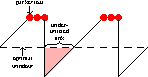
\includegraphics[width=\columnwidth]{figures/traq_illustration_too_little.pdf}
\caption{If the buffer is too small, loss-based \glspl{cca} will not be able to fully utilize the link since they send too few data following the multiplicative decrease that occurs after packet loss.}
\label{fig:tooLittle}
\end{figure}

\begin{figure}[h]
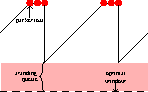
\includegraphics[width=\columnwidth]{figures/traq_illustration_too_much.pdf}
\caption{If the buffer is too large, loss-based \glspl{cca} will keep a unnecessary standing queue. This queue is unnecessary since it is not generally required to achieve full link utilization.}
\label{fig:tooMuch}
\end{figure}

Since the goal of our algorithm is to achieve optimal throughput irrespective of the \gls{cca}, we aim to avoid the scenario depicted in \autoref{fig:tooLittle}: Here the buffer is too small, meaning that the \glspl{cca} never manages to achieve full utilization and periodically underutilizes the link, leading to, for example, a user waiting longer for a software update to finish or a video game to download on their video game console. 

The other case we want to avoid is a persisting standing queue, as depicted in \autoref{fig:tooMuch}: In this case the buffer is too large meaning that optimal throughput is achieved but at the same time that an unnecessarily long standing queue is maintained. This oversized queue leads to \gls{rtt} being larger than necessary and can result in unresponsive applications and reduced Quality of Experience. Furthermore, the buffer space has to be allocated in the bottleneck device and keeps the memory from serving a more useful purpose. 

These considerations lead us to designing an algorithm that dynamically measures the \gls{cca} and adapts the buffer size to reach our goal of maximum throughput and minimal delay. The basic functionality of this algorithm would be to
\begin{enumerate}[topsep=0pt,wide,labelwidth=!,labelindent=0pt]
\item observe the \gls{cca} for a certain measurement period and then
\item increase or decrease the buffer size depending on whether the scenario of \autoref{fig:tooLittle} or \autoref{fig:tooMuch} is true. 
\end{enumerate}
The tricky thing about this is to define the measurement period: As \autoref{fig:tooLittle} and \autoref{fig:tooMuch} show, we would like to use the measurement period that is the longest period between two packet losses. If this period is observed, it is possible to compute the standing queue as simply the minimum queue observed in this interval. For example, if the minimum queue is 3 packets it means, that there is a standing queue of 3 packets and the algorithm will reduce buffer size by 3 to eliminate the unnecessary queuing. On the other side, if the buffer is too small, the algorithm computes how long the link was underutilized and how many packets could have been transmitted during the idle period. The buffer size is then increased by this number of packets. 

The problem is now the following: If the measurement period is mistakenly not the longest interval shown in the figure, but the interval between two adjacent packet losses, the algorithm would assume an enormous standing queue and drastically reduce the buffer to be close to zero. This would then lead to severe underutilization afterwards. 

The solution is thus to use a \textit{\gls{gi}}: The algorithm always waits for a specified minimum amount of time, picks the longest interval without packet loss in this guard interval and then applies its logic to reduce the standing queue on this \textit{\gls{li}}. We dynamically compute the \gls{gi} as a multiple (parameter of our algorithm) of the previous \gls{li} (\autoref{fig:intervals}): 

\begin{figure}[h]
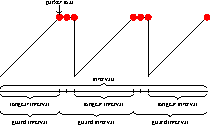
\includegraphics[width=\columnwidth]{{{figures/traq_intervals}}}
\caption{Illustration of the interval mechanism used by our \gls{qdisc} with a multiplier of $\frac{1}{2}$. Each \textit{guard interval} (GI) contains one or more intervals of which the longest one is considered the \textit{longest interval} (LI). The \gls{gi} is always at least the length of the previous \gls{li} times the multiplier. A \gls{gi} ends at the first packet loss after that is after the previous \gls{li} times the multiplier.}
\label{fig:intervals}
\end{figure}

For example, we choose the multiplier to be $\frac{1}{2}$. Now, if the \gls{li} is in the previous \gls{gi} was 100\,ms, then the next \gls{gi} is at least $\frac{1}{2} 100\,ms$. During the \gls{gi} we monitor all intervals and if the current interval is the longest one, it becomes the new \gls{li}. The \gls{gi} ends when the first packet loss occurs after the end of the \gls{gi}. 

\begin{algorithm}[h]
\caption{Procedure that is executed when a new packet is received to be enqueued.}
\label{alg:enqueue}
\begin{algorithmic}[1]%
%\algrestore{palalg}
\Function{enqueue}{new\_packet}
	\If{queue is full}
		\If{link was idle during this interval $\land$ the buffer wasn't already enlarged in this interval $\land$ this is not the first interval of this flow}
			\State buffer\_size $\gets$ buffer\_size + (packets\_transmitted\_in\_current\_interval / time\_active $\times$ time\_idle)
			\State add new\_packet to queue
		\ElsIf{the buffer was enlarged in this interval $\lor$ this is the first interval of this flow}
			\State start a new interval
			\State start a new \gls{gi}
			\State drop new\_packet
		\ElsIf{current\_time $\geq$ end\_the\_current\_\gls{gi}}
			\If{there was a standing queue in the \gls{li} of the \gls{gi}}
				\State buffer\_size $\gets$ buffer\_size - standing\_queue
			\EndIf
			\State start a new interval
			\State start a new \gls{gi}
			\State drop new\_packet
		\Else
			\State start a new interval
			\State drop new\_packet
		\EndIf
	\Else
		\State add new\_packet to queue
	\EndIf
\EndFunction
\end{algorithmic}
\end{algorithm}
Almost all of the logic of our algorithm is executed when a new packet is received to be enqueued. The full algorithm is depicted as \autoref{alg:enqueue}.

\subsection{Choice of the multiplier}

The purpose of the multiplier, which is used to multiply the \gls{li} of previous \gls{gi} to define the new \gls{gi}, is to prevent that the short gap between two subsequent packet losses is is used as the interval to determine whether the buffer size has to be adapted. This means that the multiplier must be large enough so that it allows to ``jump'' over the packet losses that occur when the buffer is full. For Reno and Cubic, the loss-free period is very large compared to the period during which packet loss occurs. Specifically, the period with packet loss has the length of one \gls{rtt} since Reno and Cubic reduce their sending rate as soon as packet loss occurs, thus ending the packet loss. This means that the multiplier can be very small in order to work for these \glspl{cca}. We conducted experiments with the multiplier being $0.5$ and have never encountered the problem that the interval between adjacent packet losses is considered the longest interval and that the buffer is cut to virtually nothing because a standing queue is assumed. However, BBR~v1 uses a completely different approach compared to Reno and Cubic to probe for bandwidth: It periodically increases its sending rate and then reduces it again to see if it can achieve more throughput. This happens with the following pattern: $[\frac{5}{4},\frac{3}{4},1,1,1,1,1,1]$. The sending rate is increased to probe for more bandwidth, then decreased to reduce the standing queue potentially formed and after that BBR is simply keeping the sending rate to match the estimated bandwidth. Each of these eight phases lasts one \gls{rtt}. BBR uses a random cyclic permutation of this pattern with the only condition being that it cannot start with $\frac{3}{4}$. The following pattern could thus occur: $[1,1,1,1,1,1,\frac{5}{4},\frac{3}{4},\frac{5}{4},\frac{3}{4},1,1,1,1,1,1]$. If the \gls{gi} ends after the first 6 phases and also the \gls{li} was these six phase, with a factor of $0.5$, the next \gls{gi} would thus end at the end of phase 8. Then, the \gls{li} would be 8th cycle. The next \gls{gi} would then be of the duration of $0.5$ phases and would then end in the middle of cycle 9. This would be erroneous because this is a probing phase during which packet loss occurs. The aforementioned problem of erroneously and significantly reducing the buffer could thus occur. This means that for BBR~v1 the multiplier must be larger than 1 since it can happen that non-probing phases are followed by probing phases of the same length. From these considerations it follows that for our experiments we generally use a multiplier of $1.25$. The behavior is different for BBR~v2 which drastically changed the probing phase and now consists of a random 2-3\,s phase of constant sending rate (cruising) followed by a quick probing phase followed by a decrease phase \cite{cardwell_bbr_2019-1,cardwell_bbr_2019}. We thus conjecture that a multiplier of $0.5$ is sufficient for BBR~v2. However, we could not finally confirm this since BBR~v2 is still not completely finished. 

\subsection{Maximum buffer increase}

Another potential problem is the following: If the link speed suddenly increases drastically, our algorithm would sharply increase the buffer size. In this case it can happen that the buffer becomes much too large. We thus limit the maximum buffer increase to be 2 times the previous buffer size. This parameter is only relevant in the case of a sudden increase of available bandwidth or if a flow's throughput is application limited and not during stable state behavior. 

\subsection{Maximum \gls{gi}}

One more challenge is posed by the following consideration: If a delay-based \gls{cca} is in its stable state, no packet loss should occur. The \gls{li} could thus become very large (like tens of seconds) and also the next \gls{gi} would be extremely large. This can be a problem if a delay-based \gls{cca} like Vegas \cite{brakmo_tcp_1995} is used for a long flow and then after several seconds, the bandwidth drastically lowers. Then suddenly packet loss could occur but the \gls{gi} would be so long that nothing would happen for a long time. To counter this, we add a parameter that specifies the maximum duration of the \gls{gi}. We set this parameter to 1\,s. This means that we also assume that no flows are handled by our \gls{qdisc} which have an \gls{rtt} larger than 1\,s. Another possibility for setting this parameter is to set it to a multiple of the \gls{rtt}, for example 2, 4 or 8 times the most recent \gls{rtt}. \gls{rtt} could be measured using TCP timestamps \cite{borman_tcp_2014} in case of TCP flows or the spin bit \cite{kuhlewind_quic_2018} for QUIC. 

\section{Implementation}

We implement our \gls{qdisc} as an extension of the ``fq'' \gls{qdisc} \cite{dumazet_pkt_sched:_2013}. This means that when using our \gls{qdisc} also all features offered by fq are available. We add three configuration parameters to the \gls{qdisc}: the multiplier (default 1.25), the maximum buffer increase (default 2.0) and the maximum \gls{gi} duration (default 1.0\,s). We make the source code of our implementation freely available to enable reproducibility and encourage experimentation: \url{https://github.com/CN-TU/traq}.

\section{Evaluation}

We evaluate our \gls{qdisc} using the \texttt{py-virtnet} (\url{https://github.com/CN-TU/py-virtnet}) toolkit to build a virtual network using Linux's network namespaces. We initialize the buffer size for our \gls{qdisc} to 100 packets per flow like in fq. 

\begin{figure}[h]
%\subfloat[Throughput of the fq \gls{qdisc}\label{fig:fqThroughput}
%]{
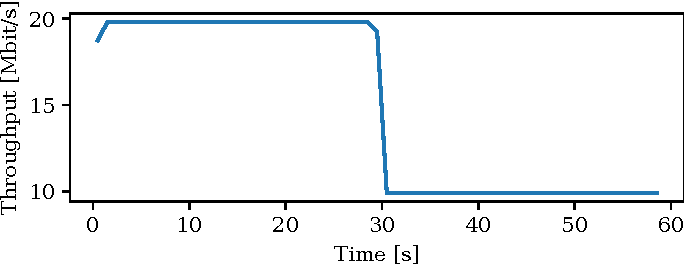
\includegraphics[width=\columnwidth]{{{../plots/throughput_1_fq_cubic_10_20_60_0.5_bw_1571240937211.pcap}}}
%}{}
%\subfloat[Delay of the fq \gls{qdisc}.\label{fig:fqDelay}
%]{
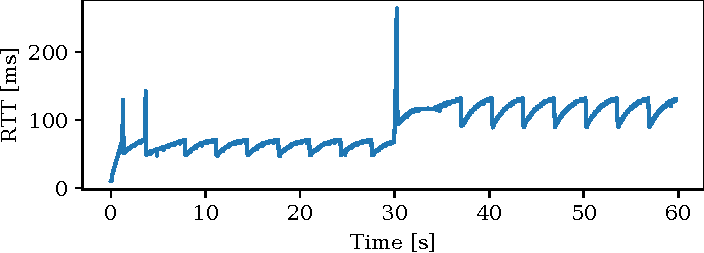
\includegraphics[width=\columnwidth]{{{../plots/rtt_1_fq_cubic_10_20_60_0.5_bw_1571240937211.pcap}}}
%}{}
\caption{Throughput and delay of a Cubic flow that is managed by fq at the bottleneck. The initial bandwidth is 20\,Mbit/s but it is halved after 30\,s. The delay is 10\,ms. It is clear that there is a standing queue and after the bandwidth halves, the minimum delay is 100\,ms even though 10\,ms would be the possible.}
\label{fig:fq}
\end{figure}

\begin{figure}[h]
\subfloat[Throughput of our \gls{qdisc}\label{fig:cnThroughput}
]{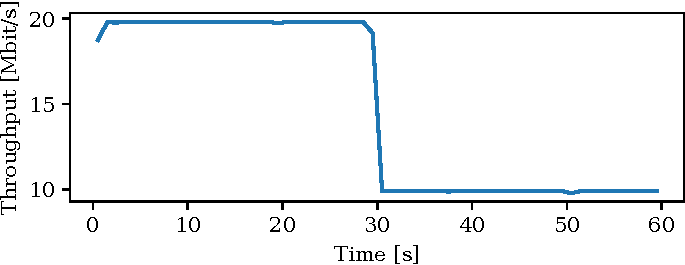
\includegraphics[width=\columnwidth]{{{../plots/throughput_1_cn_cubic_10_20_60_0.5_bw_1571241047054.pcap}}}}{}
\subfloat[Delay of our \gls{qdisc}.\label{fig:cnDelay}
]{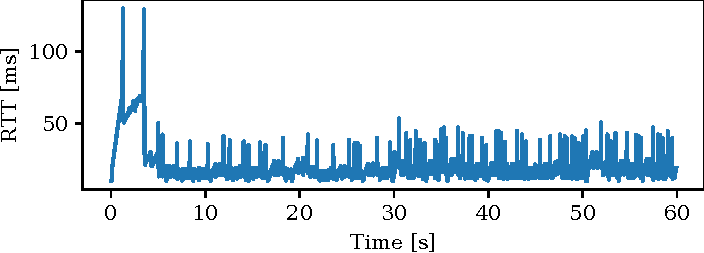
\includegraphics[width=\columnwidth]{{{../plots/rtt_1_cn_cubic_10_20_60_0.5_bw_1571241047054.pcap}}}}{}
\caption{Throughput (\ref{fig:cnThroughput}) and delay (\ref{fig:cnDelay}) of a Cubic flow that is managed by our \gls{qdisc} at the bottleneck. The initial bandwidth is 20\,Mbit/s but it is halved after 30\,s. The delay is 10\,ms. Our \gls{qdisc} manages to keep the queuing delay minimal while achieving the same throughput as with an oversized buffer.}
\label{fig:cn}
\end{figure}

\begin{figure}[h]
\subfloat[Throughput of our \gls{qdisc}\label{fig:cnThroughput2}
]{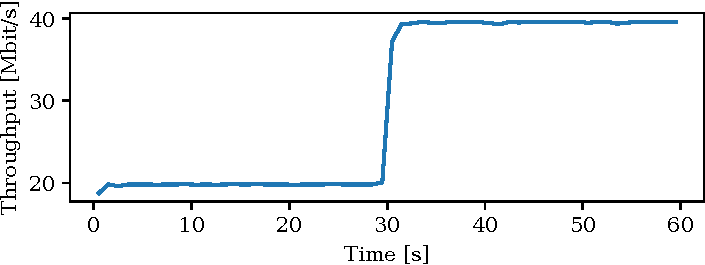
\includegraphics[width=\columnwidth]{{{../plots/throughput_1_cn_cubic_10_20_60_2.0_bw_1571241151290.pcap}}}}{}
\subfloat[Delay of our \gls{qdisc}.\label{fig:cnDelay2}
]{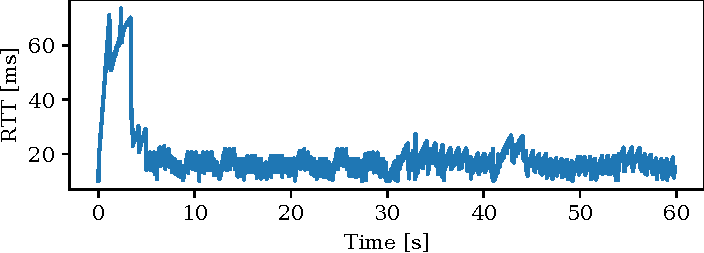
\includegraphics[width=\columnwidth]{{{../plots/rtt_1_cn_cubic_10_20_60_2.0_bw_1571241151290.pcap}}}}{}
\caption{Throughput (\ref{fig:cnThroughput2}) and delay (\ref{fig:cnDelay2}) of a Cubic flow that is managed by our \gls{qdisc} at the bottleneck. The initial bandwidth is 20\,Mbit/s but it is doubled after 30\,s. The delay is 10\,ms. Also a sudden large increase of bandwidth is handled well by our \gls{qdisc}.}
\label{fig:cn2}
\end{figure}

First we evaluate if our \gls{qdisc} is able to maintain a small buffer like it is necessary in case of small \glspl{bdp}. As can be seen in \autoref{fig:fq} the regular fq qdisc maintains a standing queue and unnecessarily leads to a significant increase in \gls{rtt} (100\,ms minimum, when the real minimum is 10\,ms). In contrast, \autoref{fig:cn} maintains the full throughput while at the same time keeping the delay minimal and not keeping a standing queue. Also, when drastically changing the bandwidth by halving it (\autoref{fig:cn}) or doubling it (\autoref{fig:cn2}) our \gls{qdisc} rapidly adapts to the new conditions and returns to the optimum state. 

\begin{figure}[h]
\subfloat[Throughput of the fq\_codel \gls{qdisc}\label{fig:fqCodelThroughputLong}
]{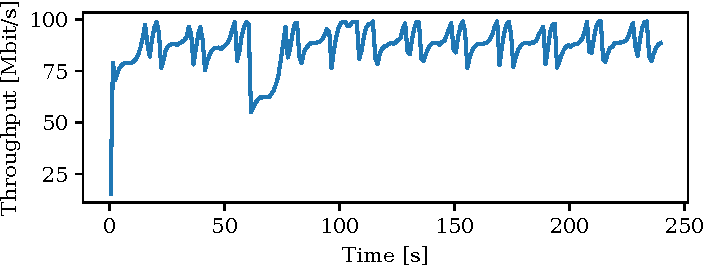
\includegraphics[width=\columnwidth]{{{../plots/throughput_1_fq_codel_cubic_100_100_240_1.0_bw_1571244312838.pcap}}}}{}
\subfloat[Delay of the fq\_codel \gls{qdisc}.\label{fig:fqCodelDelayLong}
]{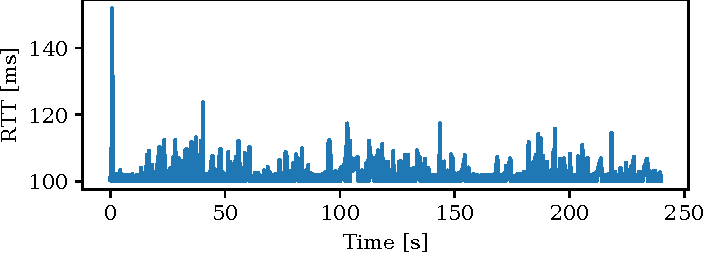
\includegraphics[width=\columnwidth]{{{../plots/rtt_1_fq_codel_cubic_100_100_240_1.0_bw_1571244312838.pcap}}}}{}
\caption{Throughput (\ref{fig:fqCodelThroughputLong}) and delay (\ref{fig:fqCodelDelayLong}) of a Cubic flow that is managed by fq\_codel at the bottleneck. The bandwidth is 100\,Mbit/s. The delay is 100\,ms. The average \gls{rtt} is 101.61\,ms. Total throughput is 2615\,MB.}
\label{fig:fqCodel}
\end{figure}

\begin{figure}[h]
\subfloat[Throughput of our \gls{qdisc}\label{fig:cnThroughputLong}
]{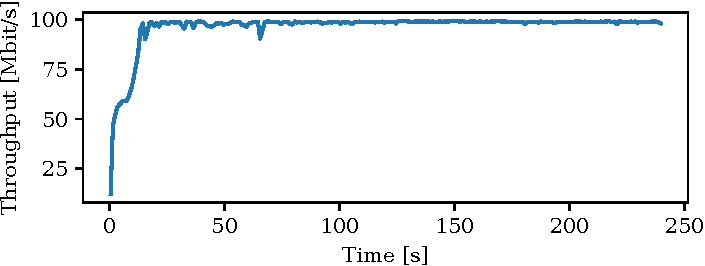
\includegraphics[width=\columnwidth]{{{../plots/throughput_1_cn_cubic_100_100_240_1.0_bw_1571244036720.pcap}}}}{}
\subfloat[Delay of our \gls{qdisc}.\label{fig:cnDelayLong}
]{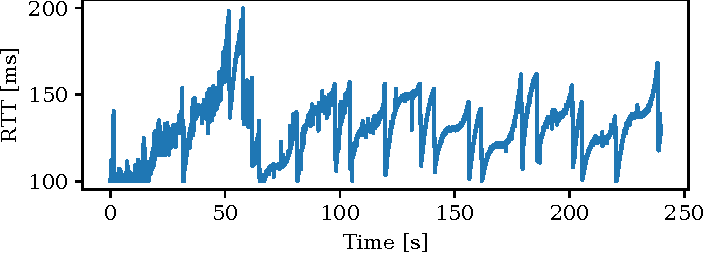
\includegraphics[width=\columnwidth]{{{../plots/rtt_1_cn_cubic_100_100_240_1.0_bw_1571244036720.pcap}}}}{}
\caption{Throughput (\ref{fig:cnThroughputLong}) and delay (\ref{fig:cnDelayLong}) of a Cubic flow that is managed by our \gls{qdisc} at the bottleneck. The bandwidth is 100\,Mbit/s. The delay is 100\,ms. The average \gls{rtt} is 130.36\,ms. Total throughput is 2893\,MB.}
\label{fig:cnLong}
\end{figure}

Next we compare our \gls{qdisc} against fq\_codel. Figure\autoref{fig:fqCodelDelayLong} shows that fq\_codel keeps the queuing delay under 5\,ms. Figure\autoref{fig:fqCodelThroughputLong} shows that keeping the queuing delay that low is detrimental for achieving full throughput when using the Cubic \gls{cca}. With our \gls{qdisc} we achieve throughput that is more than 10\% higher overall, while only slightly increasing the average delay. In addition to Cubic, we performed experiments with Reno. Here, over a 240\,s flow of 100\,Mbit/s with a delay of 50\,ms, our \gls{qdisc} achieves more than 20\% higher throughput than fq\_codel. The average \gls{rtt} for fq\_codel is 51.34\,ms while it is 96.78\,ms for our \gls{qdisc}.

Besides fq\_codel possibly leading to lower throughput as we have shown, another problem is that for links with a small \gls{bdp} fq\_codel can keep a standing queue akin to fq since fq\_codel only wants queuing delay to fall below 5\,ms once every 100\,ms. For example, on a link with a base \gls{rtt} of 5\,ms, fq\_codel would accept a permanent standing queue of 4.9\,ms, leading to overall \gls{rtt} being doubled, which is not required for achieving optimal throughput. 

We also ran experiments with the cake \gls{qdisc}. However, results were very similar to those of fq\_codel, which is no surprise since cake is based upon fq\_codel.

\begin{figure}[h]
\subfloat[Throughput of our \gls{qdisc}\label{fig:cnThroughputBBR}
]{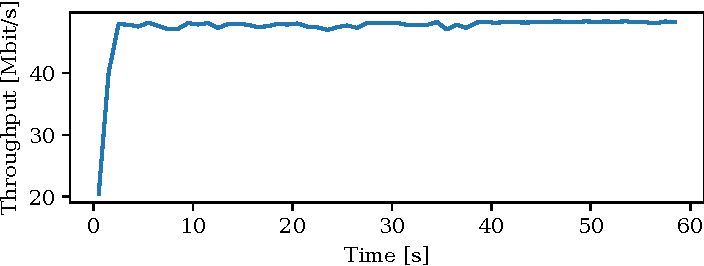
\includegraphics[width=\columnwidth]{{{../plots/throughput_1_cn_bbr_10_50_60_0.5_delay_1571288916582.pcap}}}}{}
\subfloat[Delay of our \gls{qdisc}.\label{fig:cnDelayBBR}
]{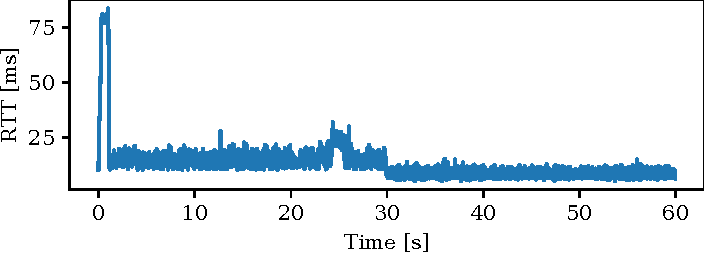
\includegraphics[width=\columnwidth]{{{../plots/rtt_1_cn_bbr_10_50_60_0.5_delay_1571288916582.pcap}}}}{}
\caption{Throughput (\ref{fig:cnThroughputBBR}) and delay (\ref{fig:cnDelayBBR}) of a BBR~v1 flow that is managed by our \gls{qdisc} at the bottleneck. The bandwidth is 50\,Mbit/s. The delay is 10\,ms and it is cut by half after 30\,s.}
\label{fig:cnBBR}
\end{figure}

Also for BBR~v1, throughput quickly reaches its maximum while no standing queue is forming \autoref{fig:cnBBR}. 

\section{Discussion}

Our goal was to design a \gls{qdisc} which achieves maximum throughput while keeping the queuing delay as small as possible. The results of the experiments, which we perform with a prototype of our \gls{qdisc}, show that there are certain common scenarios in which current state-of-the-art \glspl{qdisc} like fq, fq\_codel and cake fall short of the optimum throughput by a significant margin while our approach succeeds in leading to full utilization of the link at the bottleneck (with a potential increase in delay). Furthermore, the aforementioned \glspl{qdisc} also suffer from standing queues in scenarios with small \gls{bdp} which we can also mitigate with our approach. 

We see this work as a first step towards adaptive queuing at bottlenecks. An interesting further improvement could be to not statically initialize the buffer with a constant 100 packets but instead use experience from previous flows. Moreover, we think that a promising direction for future work might be to explore the use of reinforcement learning. Such an approach would fingerprint a flow and choose the buffer size accordingly, maximizing a chosen objective such as high throughput with minimal delay. 

\section*{Acknowledgements}
We thank Gernot Vormayr for providing us with a pre-release version of the \texttt{py-virtnet} toolkit for building virtual networks. 

\bibliographystyle{ACM-Reference-Format}
\bibliography{bibliography}

\end{document}
